%%%%%%%%%%%%%%%%%%%%%%%%%%%%%%%%%%%%%%%%%%%%
% Chapitre 6
%%%%%%%%%%%%%%%%%%%%%%%%%%%%%%%%%%%%%%%%%%%%

\chapter{Cohortes de données utilisées}
\label{Chapter7} 

Dans ce chapitre, nous présentons les différentes cohortes d'images utilisées au cours de la thèse.
Nous parlons d'une cohorte, ou encore de population, lorsque les sujets inclus ont reçu un diagnostique identique.
Les images au sein d'une même population sont acquises sur le même IRM pour éviter d'accroître l'inter-variabilité des sujets.
Au cours de la thèse, plusieurs cohortes sont étudiées.
Dans un premier temps, nous utilisons des acquisitions IRM-DT de sujets sains 
pour lesquels différents types de lésions synthétiques sont introduites.
Ces simulations sont effectuées dans le corps calleux, faisceau important de la substance blanche 
qui relie de manière unidirectionnelle les deux hémisphères du cerveau 
et par conséquent qui respecte l'hypothèse d'un modèle d'ordre 2 pour le tenseur de diffusion (voir \chapref{Chapter1}).
Cette cohorte de données synthétiques est un cadre de simulation servant à la validation des méthodes de détection développées.
La connaissance exacte des zones à détecter permet de quantifier et d'évaluer les résultats obtenus.
Dans un deuxième temps, l'étude de cas cliniques réels permettent de tester la sensiblité de nos méthodes 
et de contribuer à la recherche en neurosciences.\\

% \minitoc


%----------------------------------------------------------------------------------------

\section{Données synthétiques}
Comme expliqué en introduction de ce chapitre, des données synthétiques sont générées à partir d'image IRM-DT de sujets sains.
Cette base de sujets a été acquise au CHU de Hautepierre en Alsace sur un scanner IRM Siemens (MAGNETOM Avanto) de 1.5 Tesla.
La base comprend 22 sujets ayant entre autres une image pondérée en T1 et une série d'images pondérées en diffusion avec 30 direction de gradient associés à une b-valeur de 1000 $s/mm^2$
et 2 images de base associées à une b-valeur de 0 $s/mm^2$.
Pour les images de diffusion, la résolution spatiale est de $1.8\times1.8\times3.5\ mm^3$ et les dimensions sont de $128\times128\times41$.

L'utilisation de données synthétiques peut s'expliquer en deux points.
Premièrement, dans notre cadre d'étude, nous n'avons pas accès aux vérités terrain pour de la comparaison de groupe.
Par conséquent, il est impossible d'évaluer quantitativement les différentes méthodes et de les comparer les unes aux autres.
Les données synthétiques permettent cela car les lésions sont simulées dans une zone défnie par un masque binaire choisi par l'utilisateur.
C'est ce masque qui sert de vérité terrain.
Deuxièmement, les lésions simulées sont cohérentes avec des cas réels~\cite{Harsan2006} : 
par exemple, il a été montré que la diminution de la diffusion longitudinale peut correspondre à des modifications axonales 
telles que la diminution du calibre des axones
et que l'augmentation de la diffusion radiale peut représenter une perte de myéline sur les gaines des axones 
(pour les détails struturales des axones, il faut se réferrer au \chapref{Chapter2}).


\subsection{Introduction de lésions au sein d'une population saine}
Dans ce paragraphe, nous allons voir comment les lésions sont introduites dans des images tensorielles de sujets sains 
et comment une nouvelle population composée de \og faux patients\fg est créée.

Le groupe de 22 sujets sains est séparé en deux : 
la première moitié (11 individus) est considérée comme le groupe contrôle de sujets sains alors que l'autre moitié (11 individus) représente le groupe de sujets atteints.
Les 11 images \og faux patients\fg du groupe atteint sont générées en modifiant la forme géométrique des tenseurs de diffusion 
à l'intérieur d'un masque définissant une zone particulière de la substance blanche choisie au-préalable par l'utilisateur.
Dans notre cas, nous avons choisi une segmentation du corps calleux et nous avons restreint la région en ne conservant que 
les voxels ayant une valeur de fraction d'anisotropie supérieur à $0.3$ (FA $\geq 0.3$). 
Les valeurs propres de ces tenseurs de diffusion sont extraites et modifiées suivant le type de lésion souhaité.
Un nouveau tenseur de diffusion est alors créé à partir des nouvelles valeurs prorpres.

Quatre types de lésions sont simulés en accord avec les recherches sur les modifications axonales causées par des pathologies neurodégénératives \cite{Harsan2006} : 
une augmentation de la diffusion moyenne, une augmentation de la diffusion radiale, une diminution de la diffusion longitudinale 
et enfin une modification de l'orientation de la diffusion (voir \tabref{tab:lesion}).
Le dernier type de lésions est plus un exemple que la mise en place d'un cas réel.
Une réelle modification de la diffusion principale impliquerait une déviation globale du faisceau de la substance blanche.

\begin{table}[ht]
  \centering
  \begin{tabular}{|D{0.35\textwidth}|D{0.5\textwidth}|}
      \hline
      \textbf{Type de modifications} & \textbf{Modifications sur le tenseur} \tabularnewline
      \hline
      \hline
      Augmentation de la diffusion moyenne & $\lambda'_{i} = (1 + \alpha) \lambda_{i}$ , avec $i = {1,2,3}$ \tabularnewline
      Augmentation de la diffusion radiale & $\lambda'_{i} = \lambda_{i} + \alpha \frac{\lambda_{1} - \lambda_{i}}{2}$, avec $i = {2,3}$ \tabularnewline
      Diminution de la diffusion longitudinale & $\lambda'_{1} = \lambda_{1} - \alpha (\lambda_{1} - \lambda_{2})$ \tabularnewline
      Modification de l'orientation de la diffusion & $D' = R D R^{t}$ , avec $R$ la matrice de rotation \tabularnewline
      \hline
  \end{tabular}
  \caption{\label{tab:lesion} Equations pour simuler les 4 types de lésions (\cite{Boisgontier2012} pour les détails).
  $\lambda_{i}$ corresponds à la $i^{\text{ème}}$ valeur propre du tenseur de diffusion triée par ordre décroissant ($\lambda_{1}$ représente la valeur propre associée à la direction principale)} 
\end{table}

Un paramètre $\alpha$ permet de contrôler l'amplitude des lésions simulées, comme le montre le \tabref{tab:lesion} et la \figref{fig:lesion}.
Nous faisons varier ce paramètre de $0$ à $0.9$ par pas de $0.05$ 
et nous générons un groupe de \og faux patients\fg pour chaque valeur $\alpha$.
Ce système nous permet d'avoir un large éventail de lésion 
et ainsi de valider nos méthodes sur des lésions de petite amplitude à des lésions beaucoup plus importantes.
À la fin, notre base de données simulées est composée de $4\times19=76$ groupes de 11 images.

\begin{figure}[ht]
    \centering
    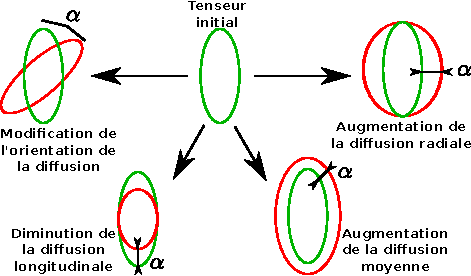
\includegraphics[scale=1.1]{Images/simulation_new.pdf}
    \caption{\label{fig:lesion}Représentation des quatre types de lésions simulées. Les tenseurs vert et rouge représentent respectivement le tenseur initial et le tenseur modifié.}
\end{figure}


\subsection{Cadre de validation : les courbes COR}
Pour évaluer les résultats des différentes méthodes, nous avons utilisé les informations fournies par l'analyse des courbes COR~\cite{Fawcett2006} 
ou en anglais, \textit{Receiver Operating Characteristics (ROC) curves}.
Cette méthode de classification permet de comparer des cartes statistiques avec la vérité terrain correspondante pour une large gamme de seuils statistiques.
Elle consiste à tracer, dans l'espace COR et pour un seuil statistique donné, 
le taux de vrais positifs (ou sensibilité) en fonction du taux de faux positifs (ou $1-\text{spécificité}$) pour.
Les définitions des différentes quantités $VPos$, $FPos$, $VNeg$ et $FNeg$ sont introduites au \chapref{Chapter4}.

\begin{align}
    \mbox{taux vrais positifs} &= \frac{VPos}{VPos + FPos}\\
    \mbox{taux faux positifs} &= \frac{VNeg}{Vneg + FNeg}
\end{align}

À cause de la bi-dimensionnalité des courbes COR, l'évaluation globale d'une méthode peut s'avérer assez complexe.
Afin de la simplifier, une information unique, sous forme d'un scalaire, est extraite de ces courbes.
Elle est obtenue en calculant l'aire sous la courbe COR, en anglais \textit{area under the curve (AUC)}.
Une valeur d'AUC de 50\% corresponds à une détection aléatoire alors qu'une AUC de 100\% représente une détection parfaite.

Pour l'évaluation des performances de nos méthodes sur données synthétiques, 
nous avons tracé les valeurs d'AUC en fonction de l'amplitude de la lésion simulée $\alpha$, et cela pour chaque type de lésions.
De cette façon, nous pouvons regarder les performances de chaque méthode autant pour des changements de diffusion importants que pour des modifications mineures.

Il est aussi important de remarquer que ce cadre de validation reste valable quelque soit la distribution statistique 
des cartes de scores obtenues en sortie du test statistique présenté en \eqref{test_stat}.
En effet, les courbes ROC ont la propriété d'être insensible au changement de distribution des tests statistiques.
Ainsi, lorsque nous comparons les méthodes de détection utilisant des métriques différentes (voir \chapref{Chapter3}-Problématiques), 
cette propriété se révèle très intéressante et permet de conserver le même cadre de validation.

Ce cadre de validation est rendu possible pour les données synthétiques car nous disposons de la vérité terrain.
Pour les études de cas cliniques, l'utilisation des courbes COR s'avère impossible 
et nous demandons alors l'expertise d'un neurologue pour analyser les résultats obtenus.


\section{Cas cliniques}
Au cours de la thèse, deux cas cliniques ont été étudiés. 
Il s'agit de pathologies neuro-dégénératives du système nerveux central chez l'homme :
\begin{itemize}
    \item la Neuromyélite Optique (NMO),
    \item la Démence à corps de Lewy, ou en agnlais \textit{Dementia in Lewy Bodies (DLB)}.
\end{itemize}


\subsection{Neuromyélite Optique (NMO)}
\subsubsection*{Pathologie}
La Neuromyélite Optique (NMO) est une maladie inflammatoire qui affecte principalement le faisceau cortico-spinal et les nerfs optiques.
Plusieurs études ont démontré des altérations dans la substance blanche de régions telles que le corps calleux, le lobe occipital et le faisceau cortico-spinal \cite{Yu2008}.
Ces lésions peuvent être associées à des troubles cliniques cognitifs, visuels et moteurs.

\subsubsection*{Données d'imagerie}
La cohorte de NMO est composé de 34 patients ayant un âge moyen de 45 ans ($\pm$ 11 ans).
Elle a été acquise sur le même IMR que la base de sujets sains, à Hautepierre, avec un scanner IRM SIEMENS de 1.5 Tesla.
Les dimensions des images sont $128\times128\times41$ et la résolution spatiale est de $1.8\times1.8\times3.5\ mm^3$.
La série d'images pondérées en diffusion se présente avec 30 direction de gradient associés à une b-valeur de 1000 $s/mm^2$
et 2 images de base associées à une b-valeur de 0 $s/mm^2$.
Pour les études effectuées sur cette cohorte, la base de sujets sains est utilisées comme groupe contrôle.
Cela est possible car les images ont été acquises sur le même scanner IRM.

\subsection{Démence à corps de Lewy (DLB)}
\subsubsection*{Pathologie}
Cette pathologie est étudiée \cite{Heitz2014}

définir le terme prodomal


\subsubsection*{Données d'imagerie}
Les données d'imagerie du protocole \og Alpha Lewy MA \fg ont été acquises sur un scanner IRM SIEMENS de 3 Tesla avec une séquence de diffusion composée de 30 gradients de diffusion 
d'une b-valeur de 1000 $s/mm^2$ et de une image de base avec une b-valeur de 0 $s/mm^2$.
Les dimensions des images sont de $96\times96\times65$ et la résolution spatiale est de $2\times2\times2\ mm^3$.

Les sujets de cette base ont été classés en \textbf{5 groupes} d'après les critères suivants :
\begin{itemize}
    \item auncun trouble cognitif : \textbf{Groupe Témoins}
    \item critères de McKeith \textit{et al.}~\cite{McKeith2005} : \textbf{Groupe DLB prodomal} et \textbf{Groupe DLB dément}
    \item critères de Dubois \textit{et al.}~\cite{Dubois2007} : \textbf{Groupe MA prodomal} et \textbf{Groupe MA dément}
\end{itemize}

Le comité d'éthique de Protections des Personne Est IV de Strasbourg a approuvé cette étude 
et les sujets inclus ont donné leur consentement par écrit.

\subsection{Cadre de validation}

\subsubsection*{Expertise médicale}

\subsubsection*{Coefficient DICE}



% Since the F-statistic maps (Eq. \ref{FisherTest2})
% may not exactly follow the same distribution for the different methods, 
% they cannot be fairly compared by using the same statistical threshold.
% To obtain comparable detection maps, the threshold is adjusted for each method to obtain the same number of detected voxels within the white matter mask.
% For these comparisons, statistical maps were thresholded in order to exhibit the 5\% most significant voxels within the white matter mask 
% and a cluster-based threshold of $N_c=10$ is then applied. 
% Additionally, we also compare the similarity of the detection maps obtained by the different methods in order to 
% highlight methods that have similar behavior.
% To this end, Dice coefficients are computed for a wide range of thresholds (adjusted for each method) in order to compare all couples of methods for different levels of sensitivity (Fig. \ref{dice}).
